
\section{User training}

\begin{figure}[H] 
	\centering
	\subfigure[Test group user training interface.]
	{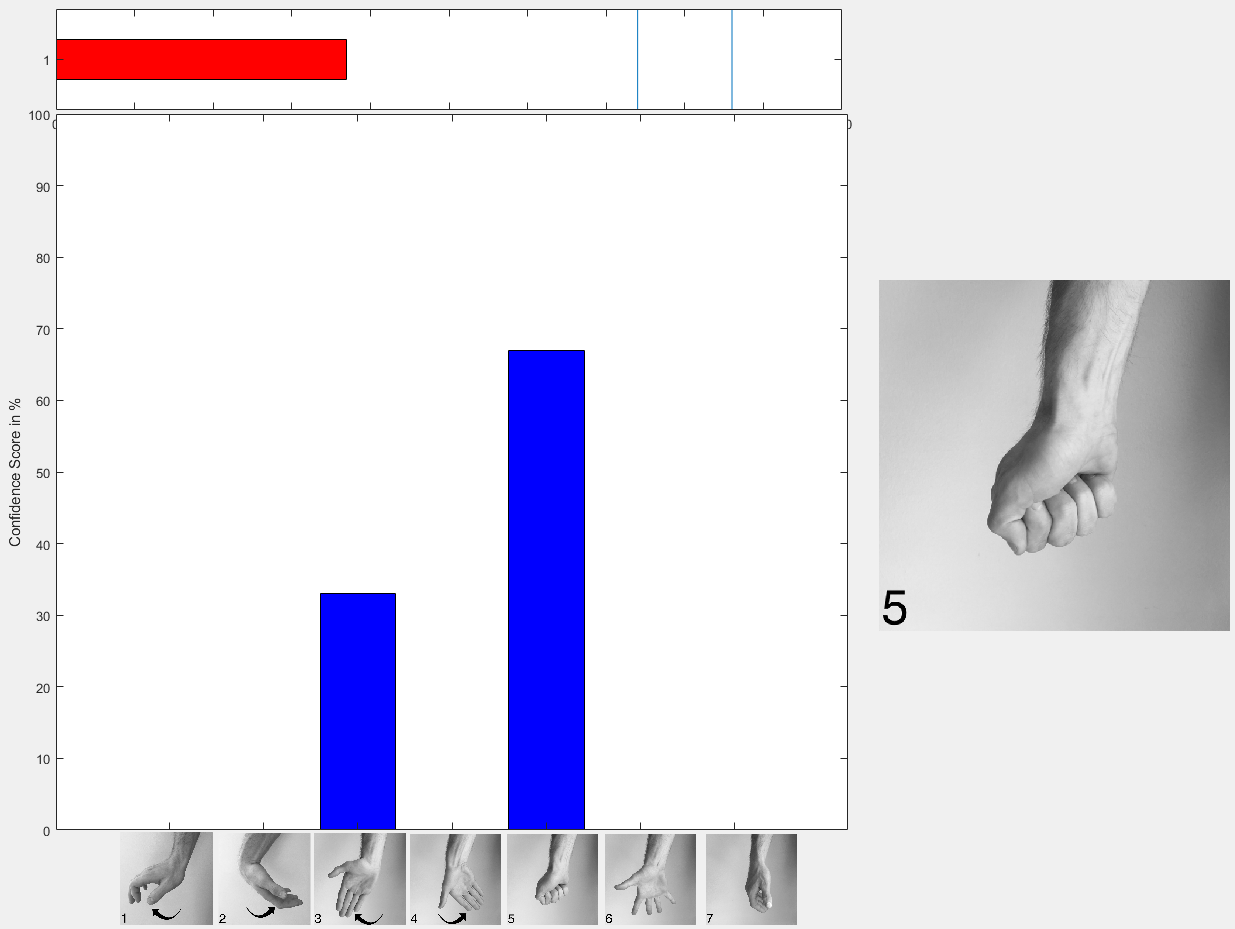
\includegraphics[width=.49\textwidth]{figures/xBackground/usertraintestGUI}}
	\subfigure[Control group user training interface.]
	{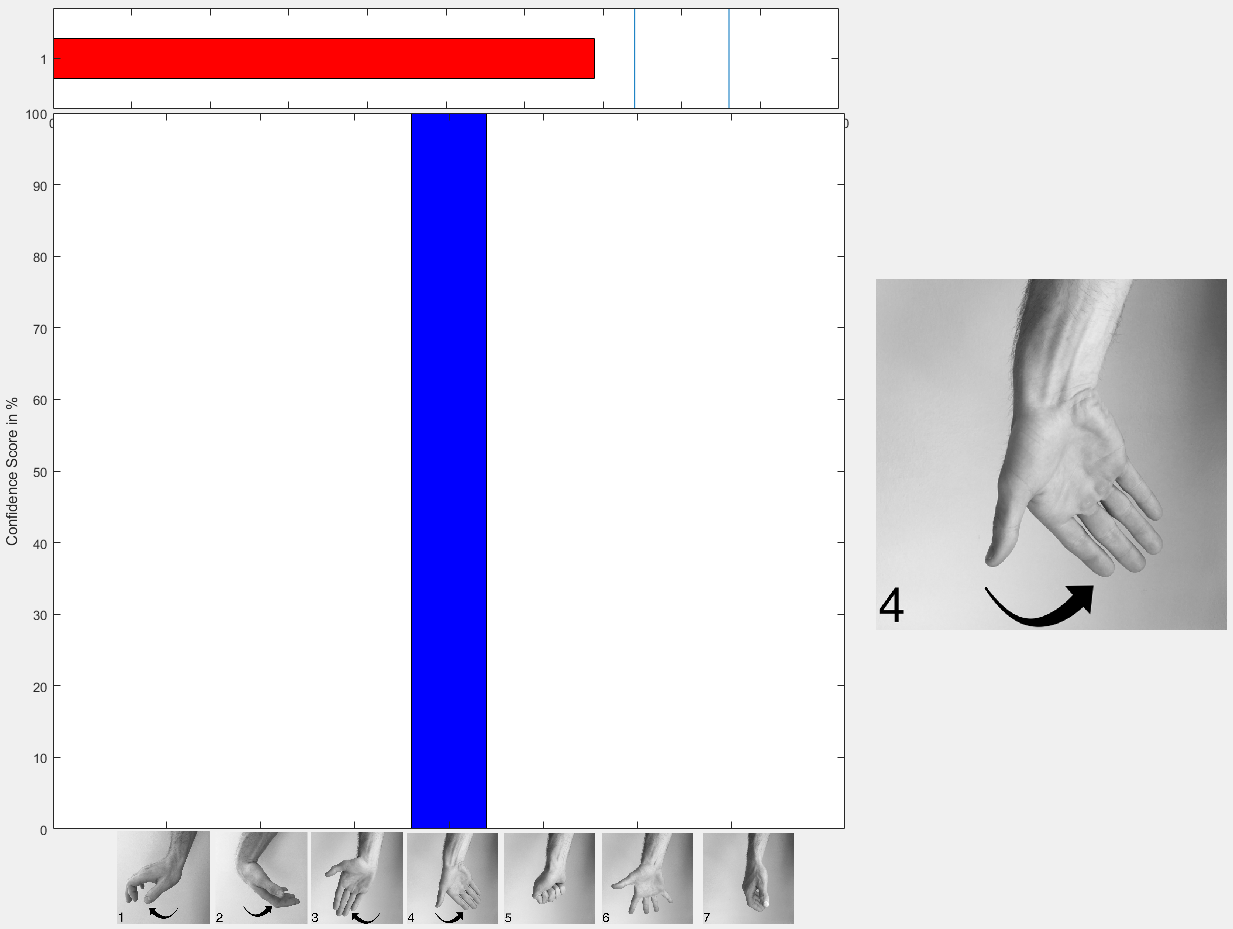
\includegraphics[width=.49\textwidth]{figures/xBackground/usertraincontrolGUI}}  
	\caption{Illustration of the user training interface for the test group (a) and the control group (b). The vertical bar plot indicates which movement is being recognized indicated by the images of each movement and the horizontal bar plot indicates contraction level. The two vertical lines in the contraction level bar plot illustrates the contraction level interval the subject must reach. The large picture of a movement on the right of the bar plot indicates which movement needs to be performed. The difference between the feedback the two subject groups receive is the information given in the vertical recognition bar plot. The control group only sees a full bar of the movement the control system recognizes the most, whereas the test groups receives the exact recognition probabilities of all movements.}
	\label{fig:feedbackGUI}
\end{figure}